% \begin{figure}[b!]
%     \centering
%     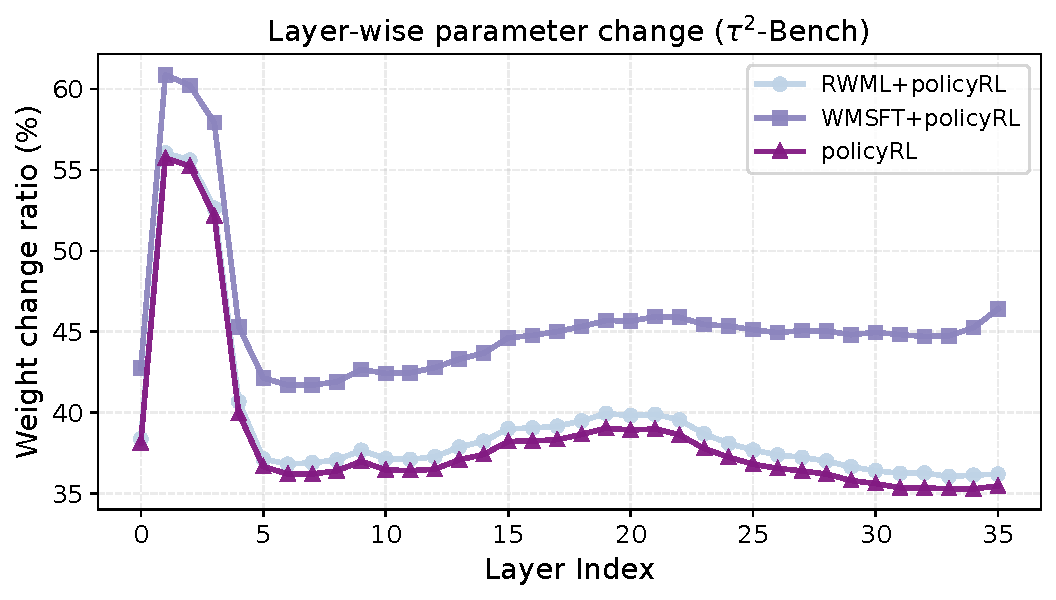
\includegraphics[width=\linewidth]{images/tau2bench_layerwise_singlecol_noWMSFT_RWML.pdf}
%     \caption{Layer-wise weight change ratios by transformer layer}
%     \label{fig:mechanism_simple}
% \end{figure}


\begin{figure*}[t]
    \centering
    \begin{subfigure}{0.48\textwidth}
        \centering
        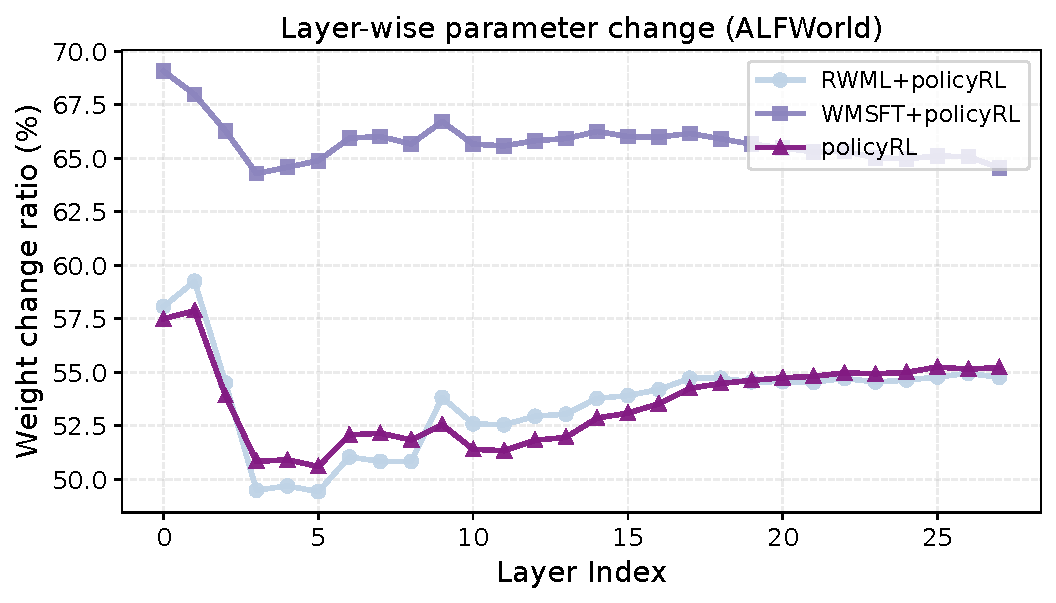
\includegraphics[width=\linewidth]{./images/alf_layerwise_singlecol_noWMSFT_RWML.pdf}
        \caption{ALFWorld}
        
        \label{fig:model_scaling_a}
    \end{subfigure}
    \hfill
    \begin{subfigure}{0.48\textwidth}
        \centering
        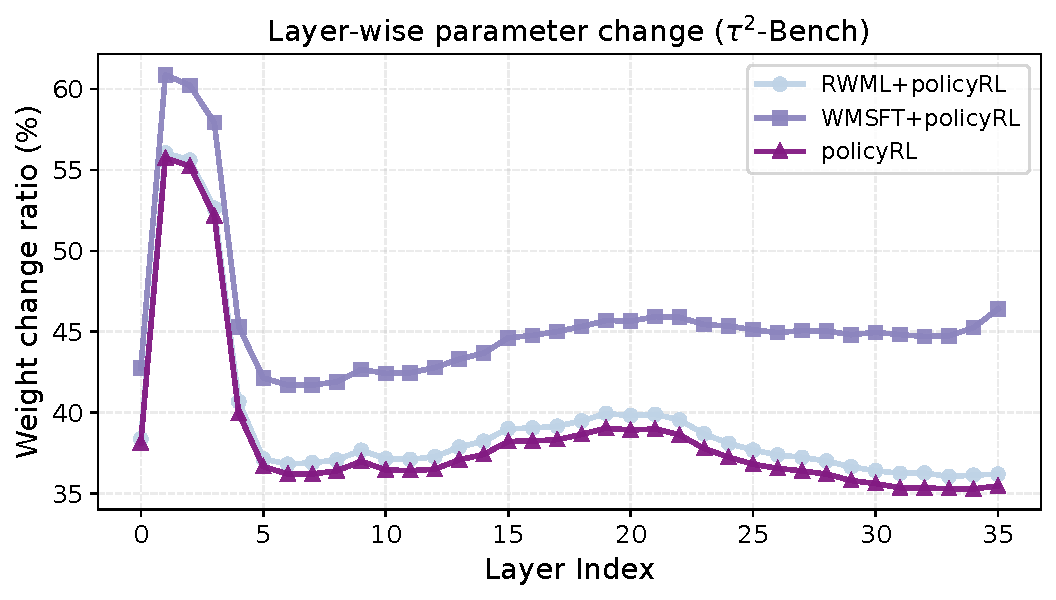
\includegraphics[width=\linewidth]{./images/tau2bench_layerwise_singlecol_noWMSFT_RWML.pdf}
        \caption{$\tau^2$ Bench}
        \label{fig:model_scaling_b}
    \end{subfigure}

    \caption{
    Comparing parameter change ratios per layer across models trained with different algorithms.
    We find \wmsftshort{}-trained models shows significantly more parameter change compare to \wmrlshort{} and \policyrl{}, potentially contributing to model forgetting in \Cref{subsec:Forgetting}.
    }
    \label{fig:mechanism_simple}
    \vspace{-2mm}
\end{figure*}